\chapter{Implementace}

\section{Vue.js framework}
Klientská část aplikace je postavena nad Vue.js frameworkem\footnote{\url{https://vuejs.org/}, \citet*{Vue}}, jež je populární JavaScriptový framework na stavbu uživatelských rozhraní. Protože některé z jeho funkcionalit byly použity v klíčových částech aplikace, je nutné čtenáře obeznámit alespoň se základním principem fungování frameworku.

\subsection{Vuex}
Vue.js framework, podobně jako konkurenční React\footnote{\url{https://reactjs.org/}} (Facebook) nebo Angular\footnote{\url{https://angularjs.org/}} (Google), využívají principu sledování stavu aplikace (jejich dat) pro automatickou změnu DOMu webové stránky. V praxi to znamená, že programátor může velice snadno napsat kód, který generuje uživatelské rozhraní na základě dat, která mohou být libovolně měněna bez nutnosti řešit problém, zda ke změně vůbec došlo a které části aplikace mají být o změně stavu informovány. Ve Vue tuto funkcionalitu zastává právě Vuex\footnote{\url{https://vuex.vuejs.org/}}, jež je možný používat samostatně.

Vuex drží stav aplikace jako jeden objekt, tedy slouží jako centrální úložiště dat pro celou aplikaci. Tento objekt se nazývá \textbf{store}. Změny ve storu mohou být sledovány Vuexem pro vykonání libovolných akcí, například překreslení textu na stránce, jež byl vykreslen Vue frameworkem.

\newcommand{\inlinecode}{\texttt}

Vrátíme-li se k původnímu příkladu, programátorovi stačí přiřadit do proměnné, jež je spravovaná Vuexem, novou hodnotu a Vuex se postará o zavolání všech komponent, které tuto proměnnou využívají a tyto komponenty na stránce překreslí původní hodnotu na novou. Překreslení přitom proběhne až poté, co skončí průběh aktuální funkce. Tohoto je docíleno pomocí \\  \texttt{Window.requestAnimationFrame()}. Díky tomuto můžeme stav v rámci průběhu jedné funkce modifikovat vícekrát se skoro nulovým dopadem na celkový výkon aplikace.

\subsubsection{Computed properties}

Kromě této funkcionality Vuex nabízí takzvané \textbf{gettery}, jež jsou ve Vue frameworku nazývány jako \textbf{computed properties}. Jedná se o funkce, které využívají data ze storu pro výpočet dat nových. Výhoda takovýchto getterů je ta, že Vuex dokáže výsledky těchto funkcí cachovat a přepočítává je pouze tehdy, změní-li se data původní. Interně gettery fungují tak, že při zavolání klientské funkce Vuex sleduje, které části storu byly dotázány a ty pak sleduje na změnu jež invaliduje cache konkrétního getteru. Při příštím požadavku na hodnotu se pak klientská funkce volá znovu a celá operace se opakuje.

Tyto computed properties jsou v aplikaci využívány často. Kupříkladu funkce, která počítá, zda je sousední uzel vybrán. Na takovouto hodnotu se v aplikaci můžeme ptát libovolně krát, ale počítá se pouze tehdy, když se množina sousedních uzlů vrcholu změní, nebo se změní právě označení vrcholu z množiny.

\subsubsection{Watchers}

Ve Vue lze využívat i \textbf{watch}ery, které umožňují registraci callbacku na změnu určité proměnné ve stavu. Watchery má smysl využívat tam, kde již data přestávají být spravována Vue frameworkem, tedy u knihoven třetích stran. Watchery, podobně jako překreslení komponent, jsou volány až po skončení probíhající funkce.

\subsubsection{Změna stavu}

Jak již bylo zmíněno, stav lze měnit přiřazením do proměnné, popřípadě voláním metod jako \texttt{.push()} na poli. Vuex dokáže tyto změny sledovat nahrazením původní proměnné (máme na mysli položku objektu) JavaScriptovým setterem. U polí dojde k obalení metody \texttt{.push()}, jež registruje změnu stavu.

Tento přístup má několik nevýhod, které se promítly i při vývoji klientské aplikace:
\begin{itemize}
  \item Vue není plně kompatibilní s novými \textbf{ES6 kontejnery} \texttt{Map} a \texttt{Set} a proto jsou v aplikaci používány jen v rámci lokálních proměnných a mapa je nahrazena klasickým objektem.
  \item Protože je v JavaScriptu nemožné sledovat \textbf{vytvoření nové property objektu}, musí programátor v tomto případě volat ručně \texttt{Vue.set(target, propertyName/index, value)} a \texttt{Vue.delete}, popřípadě vytvořit nový objekt, který nahradí ten původní.
  \item Je důležité mít na paměti, že data ve storu již nejsou původními objekty v pravém slova smyslu, protože veškeré fieldy a metody u objektů a polí byly nahrazeny, jak je zmíněno výše. Proto předání objektů a polí ze storu knihovnám třetích stran je nutné ošetřit \textbf{klonováním objektu}, jinak může dojít k zaseknutí aplikace.
  \item Instance tříd \textbf{knihoven třetích stran může zaseknout aplikaci}, pokud ji uložíme do storu. Bohužel, tohoto je velmi snadné ve Vue frameworku dosáhnout omylem.

  Řešením je využití problému, jež je popsán ve druhém bodě tohoto seznamu. (Ačkoli se může zdát, že se jedná o zneužití dokonalosti knihovny, je tento postup doporučován vývojáři frameworku.) Pokud chceme objektu nastavit kupříkladu instanci knihovny třetí strany, uložíme ji do \textbf{předem neinicializovaného} fieldu v metodě \texttt{mounted}. Taková proměnná pak nebude sledována a tedy nedojde k jejímu prohledání Vuexem.
\end{itemize}

\subsection{Vue framework}
Vue framework využívá takzvané komponenty. Komponentou se rozumí prvek na stránce, se kterým má smysl pracovat samostatně. Každá komponenta má vlastní HTML, CSS a JS. Komponenty se mohou do sebe zanořovat a vytvářet tak větší komponenty z menších. Příkladem může být komponenta \textit{seznam} jež dokáže na stránku vykreslit seznam prvků. Takováto komponenta by pak mohla mít podkomponenty jako \textit{prvek seznamu}.

Každé komponentě lze předat data formou \textbf{properties}, přičemž komponenta na základě těchto dat může vyrobit pod sebou další komponenty a předat jim část dat, která dostala.

Tato předávána data jsou právě data ze storu. Vue framework doporučuje, aby data, co komponenta dostane formou properties, neupravovala přímo, ale místo toho posílala události rodičovské komponentě, která data upraví. Ve své práci jsem se \textbf{rozhodl toto doporučení ignorovat}, neboť by tímto vzrostla náročnost na správu aplikace.

\begin{figure}[h]
    \centering
    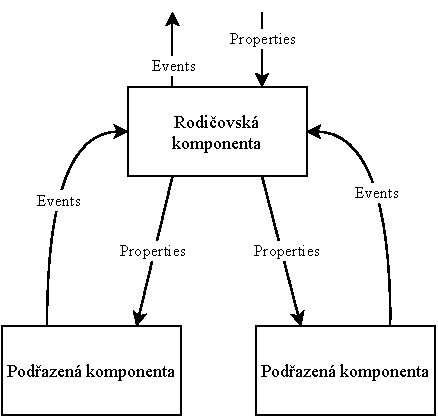
\includegraphics[width=0.5\textwidth]{media/vue.pdf}
    \caption{Doporučený způsob komunikace mezi komponentami ve Vue frameworku}
\end{figure}

\subsection{Mixins}
Někdy může být žádoucí, aby vícero komponent sdílelo stejnou množinu funkcí. V klasickém programování toto odpovídá dědičnosti tříd. Vue má takzvané Mixiny. Mixin je objekt, který komponentě dodává logiku navíc. Mixiny se dají použít jak v případě dědičnosti, kdy komponenty řeší podobný problém, tak i v případě, kdy kód jedné komponenty je příliš dlouhý a vyplatí se ho rozdělit na více částí. Mixiny totiž umožňují i vícenásobnou dědičnost.

\subsection{Loaders}
Kód Vue komponent se zapisuje do souborů s příponou \texttt{.vue}. Při sestavování aplikace se pak použije \texttt{vue-loader}, který ze souboru vyextrahuje zvlášť CSS, JS a HTML a ty předá dál na zpracování. HTML kód komponent není ve skutečnosti pravý HTML. Jedná se nadstavbu umožňující psát speciální značky, jež rozhodují kolikrát a jestli vůbec se tag na stránce vyrenderuje. Tato HTML nadstavba je pak předána \texttt{vue-template-compiler}, který vyrobí optimalizovaný JS kód jež renderuje HTML na základě stavu komponenty.

\newpage

\begin{prikl}
Ukázka jednoduché Vue komponenty \texttt{IndexedList}, která má parametr \texttt{list} očekávající pole stringů. Tato komponenta vypíše pole v odrážkovém seznamu ve formě \texttt{index: hodnota}. Komponenta se sama stará o překreslení DOMu, když se změní data. Komponentu můžeme v jiné komponentě použít vložením \texttt{<indexed-list :list="inputData" />}, kde \texttt{inputData} je proměnná obsahující pole stringů.

\begin{code}
<template>
  <ul>
    <li v-for="(item, index) in list" :key="index">
      {{index}}: {{ item }}
    </li>
  </ul>
</template>

<script lang="ts">
  import {Component, Prop} from "vue-property-decorator";
  import Vue from "vue";
  @Component
  export default class IndexedList extends Vue {
    @Prop() private list: string[];
  }
</script>

<style scoped lang="scss">
  ul {
    color: red;
  }
</style>
\end{code}
\end{prikl}

\subsubsection*{Scoped styly}

Můžeme si povšimnout \texttt{scoped} stylů v ukázce. Vue má mechanismus, že styly, které zde nastavíme, se aplikují jen na tuto komponentu. Nastavením červené barvy na seznam jsme tedy skutečně nastavili červenou barvu jen této komponentě a ostatní seznamy jsou netknuté. Toto má nespornou výhodu pokud pracujeme s velkým množstvím komponent a hrozilo by, že bychom museli používat složitě pojmenované css třídy, aby nedošlo ke kolizi.

Pokud bychom chtěli ovlivnit styly vnořených komponent a máme nastavené scoped styly, musíme použít pseudo selektor \texttt{::v-deep}, kupříkladu \\  \texttt{.actions ::v-deep .v-input--selection-controls}. Tohoto je hodně používáno, pokud je potřeba upravit styly Vuetify frameworku (viz dále).

\newpage






\section{Cytoscape knihovna}

Cytoscape.js\footnote{\url{https://js.cytoscape.org/}, \citet{10.1093/bioinformatics/btv557}} je JavaScriptová knihovna na kreslení grafů s pomocí technologie canvas\footnote{Canvas umožňuje kreslit bitmapové obrázky na stránku. Alternativou této technologie je SVG, která pracuje s vektorovými objekty. Její nevýhodou je, že pro větší grafy může limitovat výkon aplikace.}, která byla využita v tomto projektu.

Cytoscape umožňuje definovat graf pomocí vrcholů a hran, který bude vykreslen na obrazovku, kde může uživatel přesouvat jednotlivé jeho části, měnit přiblížení grafu, označovat vrcholy a podobně. Kromě toho podporuje širokou škálu možností, jak vizuálně obarvit vrcholy. Tato pravidla jsou dodávána jako style sheet a odpovídají těm, které byly zmíněné v kapitole \ref{pozadavky-visual-style-sheet}.

V knihovně lze zaregistrovat callbacky na různé události grafu a tímto jsme schopni na ně v aplikaci reagovat a propojit knihovnu i s Vue frameworkem. Umožňuje také měnit stav grafu průběžně a vytvářet tak animace, kupříkladu plynulé přiblížení grafu.

Cytoscape podporuje layoutování grafu s pomocí pluginů. V této práci byl využit Cola layout\footnote{\url{https://github.com/cytoscape/cytoscape.js-cola}}, který využívá fyzikální simulaci na esteticky příjemné uspořádání vrcholů. Původní plugin byl v mírně upraven, aby vyhovoval požadavkům na uzamykání pozic vrcholů. Kromě Coly je v aplikaci využit Dagre layout, který vrcholy uspořádá do stromové struktury.

\paragraph{Třídy} Cytoscape podporuje přidávání tříd vrcholům obdobně, jako třídy v HTML. Na tyto třídy je pak možné nastavit pravidla style sheetů. Toho je v aplikaci právě využito tak, že náhled (\ref{pozadavky-preview}) vrací seznam tříd, které budou nastaveny vrcholům a podle těchto tříd budou vrcholy barevně a jinak vizuálně rozlišeny.


\begin{prikl}
Ukázka kódu, který vytváří nový vrchol. Jak lze vidět, vytvářenému vrcholu nastavujeme ihned pozici a třídy. Kromě tříd může nést další data jako popisek (label), který se pak zobrazí jako text u vrcholu. Vrcholu jsou nastavena všechna data z \texttt{preview}, na které lze reagovat a používat je v rámci style sheetů.
\begin{code}
this.element = this.cy.add({
    group: 'nodes',
    data: {
      label: '-',
      ...clone(this.node.lastPreview),
      id: this.node.IRI
    },
    classes: this.classList,
    position,
});
\end{code}
Za povšimnutí stojí i funkce clone, která je nutná, neboť předáváme objekt z Vue frameworku.
\end{prikl}


\newpage

\section{Vuetify framework}
Na stavbu uživatelského rozhraní aplikace je pak využit Vuetify framework\footnote{\url{https://vuetifyjs.com/}}, jež je navržen pro spolupráci s Vue frameworkem. Obsahuje sadu předefinovaných komponent, které lze v aplikaci snadno použít a stavět z nich komponenty vlastní. Jedná se například o tlačítka, rozevírací seznamy, načítací lišty, dialogy, karty a další grafické prvky. Všechny komponenty Vuetify frameworku mají v názvu charakteristický prefix \texttt{v-}.

\section{Prostředí}
Klientská část aplikace je napsána v jazyce TypeScript\footnote{\url{https://www.typescriptlang.org/}}, což je typovaná nadstavba JavaScriptu. Projekt využívá balíčkovací nástroj npm\footnote{\url{https://www.npmjs.com/}} a je sestavován pomocí \texttt{@vue/cli-service}. Ten interně využívá Webpack\footnote{\url{https://webpack.js.org/}} pro sestavení celého projektu.

\subsection{Instalace}
Pro úspěšné přeložení aplikace je nutné vytvořit soubor \texttt{./conf.yaml}, který přepisuje nastavení ze souboru \texttt{./conf.default.yaml}. V tomto souboru lze nastavit výchozí jazyk aplikace, výchozí IRI meta konfigurace a URL adresu, kde se nachází server.

Pro přeložení projektu je pak nutné spustit
\begin{enumerate}
  \item \texttt{npm install} pro stažení a případnou aktualizaci balíčků, na kterých aplikace závisí.
  \item \texttt{npm run build} pro přeložení projektu.
\end{enumerate}

Výsledné soubory jsou umístěny v adresáři \texttt{./dist} včetně souboru \texttt{index.html}, odkud se aplikace spouští. Webový server by tedy měl odkazovat právě do tohoto adresáře.

\subsection*{Lokalizace aplikace}
Aplikaci lze přeložit do více světových jazyků přidáním souboru \\\texttt{<jazykový-kód>.yaml} do adresáře \texttt{./locales}. Soubor vytvořte jako kopii souboru \texttt{en.yaml}, jež obsahuje anglické překlady. Aplikaci pak stačí znova přeložit a vytvořený jazyk bude v aplikaci dostupný.

\newpage

\subsection{Adresářová struktura}
\dirtree{%
.1 /.
.2 dist \DTcomment{Adresář s vyrobenými .js a .css soubory. Obsahuje také výchozí index.html soubor.}.
.2 locales \DTcomment{Adresář s .yaml překlady aplikace.}.
.3 en.yaml \DTcomment{Anglický překlad a referenční soubor pro překlady do jiných jazyků.}.
.2 public \DTcomment{Adresář se statickými soubory.}.
.3 index.html \DTcomment{Šablona pro soubor index.html.}.
.2 src.
.3 @types \DTcomment{Definice typů pro knihovny, jež nemají oficiální typy pro Typescript.}.
.3 component \DTcomment{Obsahuje Vue komponenty.}.
.4 filter \DTcomment{Adresář s pomocnými komponentami pro filtry.}.
.4 graph \DTcomment{Adresář s komponentami pro práci s grafem.}.
.4 helper \DTcomment{Adresář s pomocnými komponentami, jež jsou použitelné v rámci celé aplikace.}.
.4 side-panel \DTcomment{Adresář s komponentami pro pravý boční panel.}.
.4 Application.vue \DTcomment{Top level Vue komponenta. Zde se vše registruje.}.
.3 configurations \DTcomment{Obsahuje logiku pro správu konfigurací a meta konfigurací.}.
.3 file-save \DTcomment{Interface pro třídy které obsahují uložitelná data.}.
.3 filter \DTcomment{Logika filtrování a jednotlivé filtry na skrývání uzlů.}.
.4 filters \DTcomment{Obsahuje adresáře s jednotlivými filtry.}.
.3 graph \DTcomment{Třídy reprezentující lokální graf.}.
.3 layout \DTcomment{Logika layoutů.}.
.4 layouts \DTcomment{Obsahuje adresáře s jednotlivými layouty.}.
.3 remote-server \DTcomment{Třídy pro stahování dat ze vzdáleného serveru.}.
.3 searcher \DTcomment{Logika vyhledávání.}.
.4 searchers \DTcomment{Obsahuje jednotlivé vyhledávače.}.
.3 LiteralTranslator.ts \DTcomment{Pomocná metody pro překlad.}.
.3 conf.ts \DTcomment{Pomocný export soubor pro konfiguraci.}.
.3 i18n.ts \DTcomment{Inicializuje překlad aplikace.}.
.3 main.ts \DTcomment{Počáteční soubor aplikace.}.
.2 conf.default.yaml \DTcomment{Výchozí nastavení aplikace.}.
.2 conf.yaml \DTcomment{Uživatelem předefinované nastavení aplikace.}.
.2 package.json \DTcomment{Balíčky pro NPM. Obsahuje seznam závislostí aplikace.}.
.2 tsconfig.json \DTcomment{Konfigurační soubor pro Typescript.}.
.2 vue.config.js \DTcomment{Konfigurační soubor pro balíčky aplikace.}.
}

\newpage


\section{Programátorská dokumentace}
V této sekci budou postupně rozebrány klíčové třídy a komponenty aplikace.

\subsection{Vstupní skript a pomocné soubory}
Vstupním skriptem celé aplikace je soubor \texttt{main.ts}, ve kterém je inicializován Vuetify a Vue framework, který spouští komponentu Application, jež je výchozí komponentou celé aplikace.

V tomto souboru je také includován soubor \texttt{LiteralTranslator.ts}, který přidává pomocné globální metody (v rámci Vue frameworku jsou dostupné pod \texttt{this}) pro překlad literálů z grafu.

\begin{itemize}
  \item \texttt{\$t_literal(translations): string|undefined} - Očekává objekt \\popsaný v kapitole \ref{jazykova-podpora} a vybere z něj nejvhodnější překlad podle pravidel popsaných ve zmíněné kapitole. Vrací \texttt{null}, pokud žádný překlad není.

  \item \texttt{\$te_literal(translations): boolean} - Vrací true, pokud by předchozí metoda našla překlad.

  \item \texttt{\$i18nGetAllLanguages(): string[]} - Vrací jazyky, které jsou požadovány ze serveru. Pokud se jazyk aplikace změní a na již stažená data vrátí \texttt{\$te_literal} false, pak se data stáhnou znovu s již správným jazykem. Tato logika je zatím implementována pouze u meta konfigurací a konfigurací.
\end{itemize}

\subsection{Komponenta Application}\label{komponenta-application}
Jedná se kořenovou komponentu celé aplikace, která drží základní třídy a moduly a řídí logiku celé aplikace. Tato komponenta registruje veškeré dialogová okna a grafické prvky.

Pro debugování aplikace je komponenta přístupná pod \texttt{window.kgvb} a je tedy možné zasahovat do jakékoli části aplikace.

Mezi důležité fieldy patří (veškeré tyto třídy budou popsány dále v textu):
\begin{itemize}
  \item \texttt{server: RemoteServer} - Třída komunikující se serverem. Obsahuje metody, které zavolají na serveru konkrétní požadavek a vrátí výsledek ve správném interface nebo false, pokud nastala chyba.
  \item \texttt{configuration: Configuration} - Aktuální konfigurace grafu ve smyslu konfigurace z kapitoly \ref{pozadavky-konfigurace}.
  \item \texttt{graph: Graph} - Aktuální graf jež závisí na \texttt{configuration}.
  \item \texttt{areaManipulator: GraphAreaManipulator} - Třída, která obsahuje \\ metody pro práci s grafovou oblastí jako přibližování, přesouvání pohledu atp.
  \item \texttt{manipulator: GraphManipulator} - Třída, která obsahuje metody pro složitější práci s grafem. Na rozdíl od \texttt{Graph}, metody v této třídě více odpovídají akcím uživatele a obvykle volají další moduly jako \texttt{LayoutManager}.
  \item \texttt{viewOptions: ViewOptions} - Jednoduchá třída mající stav, jak pohlížet na graf. Řeší, zda u hran mají být popisky a zda vůbec mají být hrany viditelné. U vrcholů pak řeší také viditelnost popisků a zda se mají zobrazit jako malé tečky.
  \item \texttt{filter: FiltersList} - Modul řešící filtrování.
  \item \texttt{layouts: LayoutManager} - Modul řešící layoutování grafu v závislosti na určitých akcích uživatele.
  \item \texttt{configurationManager: ConfigurationManager} - Drží všechny načtené konfigurace a meta konfigurace ze serveru.
  \item \texttt{visualStyleSheet: ResponseStylesheet} - Aktuální style sheet pro \\ Cytoscape knihovnu.
  \item \texttt{graphSearcher: GraphSearcher} - Třída schopna vyhledávat vrcholy v grafu a z autocomplete souborů, jež jsou specifikovány v konfiguraci.
\end{itemize}

\begin{figure}[h]
    \centering
    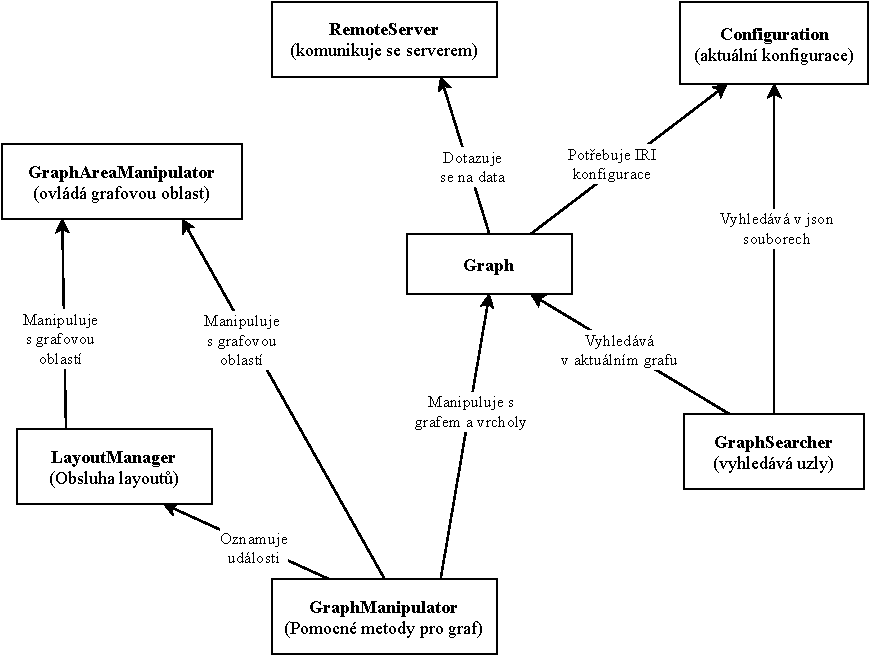
\includegraphics[width=0.8\textwidth]{media/dependencies.pdf}
    \caption{Závislosti jednotlivých tříd aplikace na sobě. Tato závislost přibližně odpovídá závislosti modulů znázorněné na obrázku \ref{fig:module-dependencies}.}

\end{figure}

\subsubsection{Závislost modulů}

Značná část modulů v aplikaci je závislá na jiných. Kupříkladu \texttt{Graph} je závislý na \texttt{RemoteServer} a částečně na \texttt{Configuration}. Na třídě \texttt{Graph} pak závisí \texttt{GraphAreaManipulator} na které závisí \texttt{GraphManipulator}. Protože těchto závislostí je hodně, některé třídy byly určeny jako readonly a tedy se může měnit pouze jejich stav. Jedná se například o třídu \texttt{RemoteServer} které lze měnit URL adresu serveru. Dalšími třídami jsou \texttt{GraphAreaManipulator}, \texttt{ViewOptions}, \texttt{FiltersList}, \texttt{LayoutManager}, \texttt{ConfigurationManager}. Ostatní třídy jsou pak měněny pouze když se mění konfigurace, v tu chvíli se starý graf zahazuje a vytváří se nový.

\medskip

Mezi důležité metody patří
\begin{itemize}
  \item \texttt{async loadStylesheet()} - Načte style sheet do proměnné \\ \texttt{visualStyleSheet} podle aktuální konfigurace \texttt{configuration}.
  \item \texttt{changeConfiguration()} - Nastaví novou konfiguraci \texttt{configuration} a zavolá metodu \texttt{createNewGraph}.
  \item \texttt{createNewGraph(loadStylesheet: boolean = true)} - Na základě konfigurace \texttt{configuration} vytvoří nový, prázdný graf (startý zahodí) a nastaví závislosti mezi moduly. Tato metoda pak ještě resetuje nastavení filtrů a plátna kde se vykresluje graf.
  \item \texttt{updateGraphSearcher()} - Pomocná metoda pro \texttt{createNewGraph}, která na základě konfigurace a grafu sestaví třídu schopnou vyhledávat nové vrcholy v grafu.
\end{itemize}

Kromě těchto metod komponenta obsahuje ještě Vue metodu \texttt{mounted}, která skryje uvítací obrazovku aplikace, až se komponenta (a tedy i celá aplikace) inicializuje. Kontroluje také URL adresu, zda neobsahuje parametry \texttt{load}, \\ \texttt{meta-configuration} nebo \texttt{configuration} které přimějí aplikaci načíst graf z url, respektive načíst meta konfiguraci, respektive konfiguraci.

\subsubsection{ApplicationLoadStoreMixin}
\texttt{ApplicationLoadStoreMixin} rozšiřuje komponentu o načítání a ukládání grafu ze a do souboru.

\paragraph{askForSaveAndPerformAction(modal: boolean, callback: Function)}\mbox{}\\ Tato funkce zkontroluje, zda jsou v grafu nějaké neuložené změny a pokud ano, otevře \texttt{SaveDialog} komponentu. Podle odpovědi na dialog pak graf uloží a v případě kladného potvrzení zavolá \texttt{callback} funkci, která pak může například vytvořit nový graf. Pokud žádné změny nejsou, callback je volán okamžitě.

\paragraph{loadFromFile(file: File), loadFromUrl(url: string)} - Metoda otevře soubor, respektive soubor z URL a přečte ho jako JSON. Výsledný objekt pak předá metodě \texttt{ObjectSave::restoreFromObject}.

\paragraph{saveToFile()} - Vyrobí soubor se stavem aplikace který je možné stáhnout.

\subsection{Interface file-save/ObjectSave}
Interface \texttt{ObjectSave} předepisuje dvě metody \texttt{saveToObject(): object} a \texttt{restoreFromObject(object: any): void}, které uloží stav třídy do serializovatelného objektu, respektive tento stav obnoví. Tento interface obsahují všechny třídy jež drží stav aplikace který je třeba uložit do souboru, pokud o to uživatel požádá.

Tento interface implementuje i komponenta \texttt{Application} jež tyto metody volá na modulech a jednotlivé výsledky pak spojí do jednoho objektu (v případě metody \texttt{saveToObject}). Výsledek je pak serializován do JSONu a uložen do počítače. V opačném případě je JSON deserializován a předán metodě \texttt{restoreFromObject} která volá tuto metodu na modulech, které ji mohou volat na podtřídách.

\paragraph{Poznámka:} Je třeba mít na paměti, že metoda \texttt{saveToObject} by měla vracet plain Javascript objekt, tedy veškeré neprimitivní typy, jako objekty a pole musí být klonovány, pokud jsou ve vlastnictví Vue frameworku. Taktéž je třeba dbát na zpětnou kompatibilitu u metody \texttt{restoreFromObject}.

\smallskip

Do budoucna se nabízí tento interface rozšířit o více módů ukládání. Tento problém je popsán v poslední kapitole.

\subsection{Třída Graph}

\begin{figure}
    \centering
    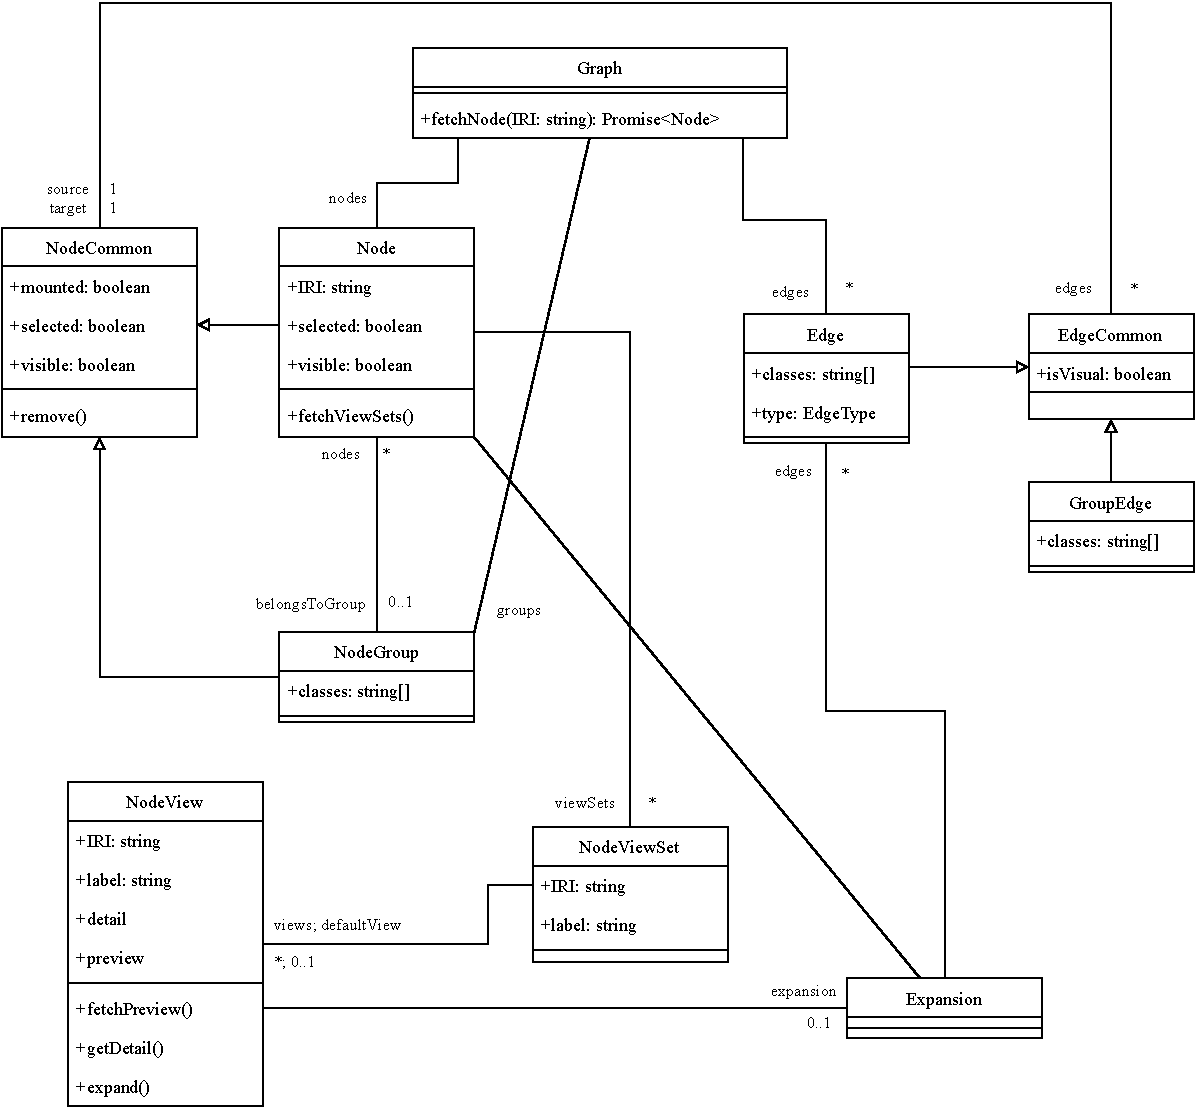
\includegraphics[width=\textwidth]{media/graph.pdf}
    \caption{Class diagram tříd, které pracují s grafem.}
\end{figure}

Třída \texttt{Graph} umístěna v \texttt{graph/} spravuje stažený graf pod konkrétní konfigurací. Závisí na \texttt{server: RemoteServer} a \texttt{configuration: Configuration}. Pokud se konfigurace mění, nebo se načítá nový graf ze souboru, je tato třída zahozena. Ačkoli třídy jako \texttt{Node} nebo \texttt{Edge} obsahují fieldy pro obsluhu viditelného grafu, třída \texttt{Graph} a ostatní nemusí být explicitně použity na vykreslení grafu na plátno, ale mohou být použity pro držení obecného grafu.

\subsubsection*{Fieldy}
\begin{itemize}
  \item \texttt{nodes} objekt tříd \texttt{Node} - Seznam všech vrcholů grafu.
  \item \texttt{edges} objekt tříd \texttt{Edge} - Seznam všech hran stažených ze serveru.
  \item \texttt{groups: NodeGroup[]} - Seznam všech neprázdných skupin vrcholů.
  \item \texttt{nodesVisual: NodeCommon[]} - Všechny \texttt{Node} a \texttt{NodeGroup}, které jsou aktuálně viditelné v grafu. \textit{Viditelnost vrcholů je popsána dále.}
  \item \texttt{groupEdges: GroupEdge[]} - Hrany které propojují skupiny uzlů nebo skupinu a normální uzel. Tyto hrany vzikly sloučením několika hran a existují pouze díky existenci nějaké skupiny vrcholů.
  \item \texttt{edgesVisual: EdgeCommon[]} - Všechny \texttt{Edge} a \texttt{GroupEdge} které jsou aktuálně viditelné v grafu. \textit{Viditelnost hran je popsána dále.}
\end{itemize}

Poslední tři zmíněné fieldy jsou gettery. Protože se aplikace často na tyto proměnné dotazuje, je využito Vuexu a tyto hodnoty jsou ve skutečnosti computed properties. Protože třída \texttt{Graph} není komponentou, má také field \texttt{vuexComponent: GraphVuex} na komponentu, která se vytvoří automaticky společně s grafem a tyto zmíněné fieldy počítá. Tak docílíme cachování těchto hodnot a k jejich přepočítání dojde pouze tehdy, změní-li se hrany, nebo vrcholy v grafu.

\subsubsection*{Metody}
\begin{itemize}
  \item \texttt{getNodeByIRI(IRI: string): Node|null} - Vrátí vrchol dle jeho IRI nebo \texttt{null} v případě, že neexistuje.

  \item \texttt{createNode(IRI: string): Node} - Vytvoří a zaregistruje nový vrchol v grafu.
  \item \texttt{createEdge(source: Node, target: Node, type: EdgeType): Edge}\mbox{}\\Vytvoří a zaregistruje novou hranu v grafu.
  \item \texttt{createGroup(): NodeGroup} - Vytvoří a zaregistruje prázdnou skupinu vrcholů.

  \item \texttt{getAllTypes(): Set<NodeType>} a \texttt{getAllClasses(): Set<string>}\mbox{}\\Pomocné metody, které projdou všechny uzly v grafu a shromáždí jejich typy, respektive třídy. Těchto metod je využíváno při filtrování, protože nejsme schopni ze serveru získat kompletní množinu typů a tříd. Metody jsou volány, když uživatel otevře okno s možnostmi filtrů.

  \item \texttt{fetchNode(IRI: string): Promise<Node>} - Vrchol je definován pouze svým IRI a tedy pro vytvoření vrcholu se aplikace nemusí ničeho dotazovat serveru. Tato metoda kromě vytvoření takového vrcholu ještě stáhne jeho \texttt{view-sets}, zvolí výchozí pohled a stáhne \texttt{preview} vrcholu. V případě, že se nepodaří stáhnout tyto informace, pak podle požadavku na vložení vrcholu z \ref{pozadavky-uzivatelske}, vrchol do grafu nebude přidán a metoda vrátí null.

  \item \texttt{getOrCreateNode(IRI: string): Promise<Node>} - Obdobná metoda \\metodě výše. Pokud uzel neexistuje, volá předchozí metodu. Pokud uzel existuje, stáhne jeho \texttt{view-sets} a \texttt{preview} obdobně jako předchozí metoda a vrátí ho.
\end{itemize}

\paragraph{Poznámka k viditelnosti} Veškeré metody, které vytvářejí vrcholy, skupiny nebo hrany, tyto prvky nevytvoří viditelnými. Aby mohl být prvek viděn v grafu, musí mu být nastaven field \texttt{mounted = true}.

\subsection{Třída NodeCommon}
Třída \texttt{NodeCommon} je společným předkem pro třídy \texttt{Node} a \texttt{NodeGroup} a zaštiťuje především jejich vizuální vlastnosti.

\subsubsection*{Fieldy}
\begin{itemize}
  \item \texttt{mounted: boolean} - Určuje, zda má být vrchol viditelný v aplikaci. Na rozdíl od ostatních úrovní viditelností je tato myšlena tak, že uzel, který má tuto hodnotu false, v grafu vůbec nefiguruje a není jej možné ani najít v jiných částech aplikace (například mezi skrytými vrcholy). Využití najde v případě, kdy server pošle více vrcholů než uživatel žádal, nebo ho lze použít v případě browsingu seznamem, který je popsán v poslední kapitole.

  \item \texttt{onMountPosition: [number, number]} - Pomocný field, který určuje, kde má být vrchol na plátně vykreslen, až bude nastaven na mounted. Souřadnice odpovídají souřadnicím používanými Cytoscape knihovnou.

  \item \texttt{visible: boolean} - Nastavuje uživatelskou viditelnost uzlu. Uživatel se může rozhodnout ručně skrýt uzel. Takový uzel si pak zachovává svou pozici na plátně a je v seznamu mezi ostatními skrytými uzly.

  \item \texttt{get isVisible: boolean} - Pomocný getter, který určí, jestli je uzel viditelný. Pro \texttt{NodeGroup} se počítá jako \texttt{visible} AND \uv{alespoň jeden vrchol skupiny je \texttt{isVisible}}.  \texttt{Node} pak viditelnost počítá jako \texttt{visible} AND \uv{žádný filtr nezakazuje jeho viditelnost}.

  \item \texttt{selected: boolean} - Pokud je vrchol vybrán, je zobrazen jeho detail v pravém panelu aplikace. Je možné vybrat více vrcholů. Vybrání vrcholů je napojeno na vybírání vrcholů na plátně. Lze vybrat i skryté vrcholy (uživatelem, nebo filtrem). Pokud vrchol není mounted, je tato hodnota ignorována.

  \item \texttt{get neighbourSelected: boolean} - Pomocný getter, který vrátí true, pokud sousední vrchol byl vybrán. Využívá se pro zvýraznění sousedních vrcholů vybraného vrcholu v grafu.

  \item \texttt{get identifier: string} - Jednoznačný identifikátor pro potřeby Cytoscape knihovny.

  \item \texttt{get selfOrGroup: NodeCommon} - Pomocný field, který vrátí buď sebe, nebo skupinu do které vrchol patří. Využití má čistě pro zjednodušení programování a využívá se například v částech kódu, kde se řeší kontrakce hran.

  \item \texttt{lockedForLayouts: boolean} - Pokud daný layout podporuje zamykání pozic vrcholů, tato proměnná určuje, jestli je jeho pozice zamčená.
\end{itemize}

\subsubsection*{Metody}
\begin{itemize}
  \item \texttt{remove()} - Smaže vrchol z grafu společně s jeho hranami. V případě skupiny smaže skupiny a vrcholy v ní.
  \item \texttt{selectExclusively()} - Nastaví \texttt{selected} pouze pro tento vrchol. V praxi to znamená, že se zobrazí detail tohoto vrcholu v pravém panelu.
\end{itemize}

\paragraph{Poznámka} Díky Vue frameworku je hodně akcí vyvoláno právě nastavením nějaké proměnné. Kupříkladu proměnná \texttt{mounted} místo metody \texttt{mount()}. Vue framework automaticky při změně takovýchto proměnných provede příslušnou akci. Tento přístup má několik výhod, kupříkladu můžeme napojit proměnnou \texttt{visible} na checkbox a tak propojit viditelnost vrcholu se zaškrtávacím políčkem v obou směrech. Nevýhoda tohoto přístupu je ta, že skutečná akce bude provedena až po skončení funkce. Pokud bychom například chtěli počkat, až se uzel namountuje a pak provést nějakou akci, musíme počkat na další AnimationFrame. Následující kód toto předvádí na akci, kdy chceme vrchol zobrazit v grafu a pak na něj přesunout pohled.

\begin{code}
node.mounted = true;
await Vue.nextTick(); // Mounting function is called
this.area.fit(node)
\end{code}

\subsection{Třída Node}
Třída \texttt{Node} rozšiřuje třídu \texttt{NodeCommon} a reprezentuje vrchol získaný ze serveru, tedy entitu z RDF databáze.

\subsubsection*{Fieldy}
\begin{itemize}
  \item \texttt{get classes: string[]} - Seznam tříd z posledního kompletního pohledu. \textit{(viz dále)}
  \item \texttt{get edges: Edge[]} - Seznam hran příslušících vrcholu.
  \item \texttt{filters} jako objekt - Objekt jehož klíčem jsou identifikátory filtrů a hodnotou je \texttt{boolean}, zda konkrétní filtr povoluje viditelnost vrcholu. Objekt je aktualizován kdykoli se změní stav vrcholu, který daný filtr využívá, nebo se změní nastavení filtrů. Všechny hodnoty nastavené na \texttt{true} jsou nutnou podmínkou viditelnosti vrcholu.
  \item \texttt{get shownByFilters: boolean} - Zdali všechny hodnoty objektu výše jsou nastaveny na true.
  \item \texttt{currentView: NodeView} - Určuje aktuální pohled na vrchol.
  \item \texttt{lastFullView: NodeView | null} - Tato proměnná odkazuje na poslední pohled na vrchol, který měl kompletní \texttt{preview}. Změna pohledu je totiž okamžitá, ale změněný pohled ještě nemusí mít stažený \texttt{preview}. To by způsobilo zbytečné \uv{blikání} vrcholu v grafu, když by uživatel měnil jeho pohledy. Na krátkou chvíli by totiž neměl žádné třídy a tedy by se vypnuly jeho styly.
  \item \texttt{viewSets} jako objekt \texttt{NodeViewSet} - Seznam view setů. Pokud view sety ještě nebyly staženy, pak je hodnota tohoto fieldu rovna \texttt{null}.
  \item \texttt{belongsToGroup: NodeGroup | null} - Určuje, zda vrchol patří do skupiny. Pokud ano, pak nebude zobrazen na plátně.
\end{itemize}


\subsubsection*{Metody}
\begin{itemize}
  \item \texttt{async fetchViewSets(): Promise<void>} - Metoda asynchronně stáhne view sety. Tato metoda (společně s dalšími) je navržena tak, že druhým voláním nezahájí druhé stahování, ale vrátí existující Promise z prvního. Takto nedojde k zatížení serveru a datových zdrojů. Ukázka metody je zobrazena an obrázku \ref{fetchViewSets}.
  \item \texttt{async useDefaultView(): Promise<NodeView>} - Metoda stáhne pohledy a nastaví výchozí, v případě že vrchol nemá nastaven žádný pohled.
\end{itemize}

\paragraph{Poznámka} Aktuální interface serveru vrací při expanzi detail vrcholů. Detail formálně patří k pohledu ale v odpovědi ze serveru není určeno, o jaký pohled se jedná. Takový pohled je pak nastaven jako aktuální, ale při volání metody \texttt{useDefaultView} bude ignorován a přepsán.


\begin{figure}
\begin{code}
private fetchViewSetsPromise: Promise<void> = null;

async fetchViewSets(): Promise<void> {
    let asynchronouslyFetchViewSets = async () => {
        let result = await this.graph.server.getViewSets(...);

        if (result) {
            this.viewSets = ...;
        }
        this.fetchViewSetsPromise = null;
    }

    if (!this.viewSets) {
        if (!this.fetchViewSetsPromise) {
            this.fetchViewSetsPromise = asynchronouslyFetchViewSets();
        }

        return this.fetchViewSetsPromise;
    }
}
\end{code}
\label{fetchViewSets}
\caption{Příklad kódu na stažení view setů. Metoda má vevnitř další metodu která je volána pouze tehdy, neskončila-li předchozí Promise. Takto zařídíme pouze jeden požadavek na server současně.}
\end{figure}

\subsection{Třída NodeGroup}
Třída \texttt{NodeGroup} rozšiřuje třídu \texttt{NodeCommon} a reprezentuje skupinu vrcholů \texttt{Node}. Aktuálně není podporováno, aby skupina obsahovala další skupiny. Všechny pomocné metody pro manipulaci v rámci skupiny pak řeší přeskupování tak, že prvně vrcholy ze skupiny odstraní a vloží je do jiné.



\subsubsection*{Fieldy}
\begin{itemize}
  \item \texttt{get classes: string[]} - Vrátí průnik tříd všech vrcholů, které obsahuje. Takto lze docílit, že skupina podobných vrcholů bude mít stejný styl jako jednotlivé vrcholy.
\end{itemize}

\subsubsection*{Metody}
\begin{itemize}
  \item \texttt{addNode(node: Node, overrideExistingGroup: boolean = false)}\mbox{}\\Vloží vrchol do skupiny.
  \item \texttt{checkForNodes()} - Pomocná metoda pro kontrolu, zda skupina vůbec nějaké vrcholy obsahuje. Pokud tomu tak není, odstraní se. Pokud obsahuje jen jeden vrchol, odstraní se a vrchol odstraní ze skupiny.
  \paragraph{Poznámka} Tato operace ve skutečnosti může být kontrolována Vue frameworkem. Nicméně kvůli jednoduchosti ruční implementace je vytváření a odstraňování skupin spravováno mimo framework.
\end{itemize}

\subsubsection{Generování GroupEdges}
\texttt{NodeGroup} seskupuje několik vrcholů a z grafového hlediska provádí jejich kontrakci. To znamená, že musíme sjednotit několik hran do jedné.

Třída obsahuje field \texttt{groupEdgesCache}, který udržuje tyto virtuální hrany. Kdykoli dojde ke změně v grafu, dojde k opětovnému přepočítání těchto virtuálních hran a pokud již existují, budou použity tyto existující. Pokud vznikne nová hrana, bude uložena do této cache a pokud nějaká hrana zanikla, bude z této cache odstraněna.

Tímto způsobem je docíleno automatického generování těchto hran, přičemž existující hrany se nemění (jejich instance zůstává stejná). Celý proces je spravován Vue frameworkem a tedy se děje automaticky.

Třída má field \texttt{get visibleGroupEdges: GroupEdge[]}, který vrací všechny hrany kromě těch, které vycházejí z jiné \texttt{NodeGroup}. Jednoduchým sjednocením pak dostaneme všechny hrany a každou právě jednou. Hrany se vypočítávají funkcí \texttt{getGroupEdgesInDirection}, která kvůli komplexnosti počítá hrany jen v jednom směru a musí se tedy volat dvakrát. Jak již bylo zmíněno, tato funkce používá cache, aby vracela již existující hrany. Výsledek funkce je pak ještě jednou cachován, tentokrát pomocí computed properties a tedy k přepočítání dojde pouze tehdy, změní-li se graf.

\subsection{Třídy EdgeCommon, Edge, GroupEdge}
Hrany RDF grafu jsou pak reprezentovány třídou \texttt{Edge} a hrany mezi skupinou a vrcholem, nebo dvěma skupinami třídou \texttt{GroupEdge}.

Společný předek předepisuje \texttt{get isVisual: boolean} který určuje, zda je hrana přítomná na plátně. Hrana je \texttt{isVisual} pokud její oba vrcholy jsou \texttt{mounted} a nepatří do skupiny. Obdobně pro \texttt{GroupEdge} je podmínka splněna pokud jsou oba vrcholy \texttt{mounted}.

\subsubsection*{Fieldy třídy Edge}
\begin{itemize}
  \item \texttt{type: EdgeType} - Typ hrany který určuje její label.
  \item \texttt{classes: string[]} - Třídy hrany.
\end{itemize}

\subsection{Třída NodeViewSet}
Třída reprezentuje view set popsaný v kapitole \ref{pozadavky-view-sets}. Jedná se o kontejner pro pohledy. Z hlediska implementace je třída velmi jednoduchá. Obsahuje seznam pohledů jako \texttt{views} a výchozí pohled \texttt{defaultView: NodeView}.

Obsahuje metodu \texttt{createView(IRI: string): NodeView}, která vytvoří \\a vhodně zaregistruje nový pohled. Protože jednotlivé pohledy jsou součástí jednoho požadavku (server na \texttt{view-sets} vrátí i pohledy) je logika vytváření pohledů ve třídě \texttt{Node}.

\subsection{Třída NodeView}
Tato třída odpovídá pohledům tak, jak jsou definovány v kapitole \ref{pozadavky-view}.

\subsubsection*{Fieldy}
\begin{itemize}
  \item \texttt{detail: DetailValue[]} - Představuje pole detailů, které lze získat ze serveru voláním \texttt{detail} a odpovídají \ref{pozadavky-detail}. Interface \texttt{DetailValue} pak obsahuje \texttt{type}, \texttt{IRI} a \texttt{value}. Aktuálně je \texttt{value} v rámci aplikace považována za textový řetězec. Do budoucna je možné aplikaci rozšít o více typů. Tomuto tématu se opět věnuje poslední kapitola.
  \item \texttt{preview: NodePreview} - Obsahuje základní informace o vrcholu, které řídí jeho vykreslení na obrazovce. Preview lze získat voláním \texttt{preview} na serveru a odpovídá definici v \ref{pozadavky-preview}.
  \item \texttt{expansion: Expansion} - Expanze dle tohoto pohledu. \textit{Třída je popsána dále.}
\end{itemize}

\subsubsection*{Metody}
\begin{itemize}
  \item \texttt{async getDetail(): Promise<DetailValue[]>} - Stáhne, uloží a vrátí detail.
  \item \texttt{async fetchPreview(): Promise<NodePreview>} - Stáhne, uloží a vrátí preview.
  \item \texttt{async expand(): Promise<Expansion>} - Provede expanzi a vrátí ji.
\end{itemize}

Všechny tři funkce mají podobnou ochranu proti opětovnému volání, jako metoda \texttt{fetchViewSets}, jejíž ukázka je na obrázku \ref{fetchViewSets}. Metoda \texttt{expand} používá třídu \texttt{Graph}, vytváří nové vrcholy a nastavuje jim \texttt{preview}. Nově vytvořené vrcholy nemají nastavené \texttt{mounted}, takže je lze snadno rozeznat a vhodně layoutovat.

\subsection{Třída Expansion}
Aktuálně třída \texttt{Expansion} je v aplikaci využívána pouze během procesu expanze. Do budoucna ji lze použít například pro znázornění vrcholů, které vznikly z jiných vrcholů v rámci expanze. Obsahuje seznam vrcholů \texttt{nodes: Node[]} a hran \texttt{edges: Edge[]}

\bigskip

Veškeré třídy zde zmíněné pro práci s grafem implementují rozhraní \\\texttt{ObjectSave} a tedy je možné na třídě \texttt{Graph} volat metody pro uložení a obnovení stavu.







\newpage

V následujících kapitolách práce bude popsáno, jak je tento modul grafu integrován do Vue frameworku tak, aby se samy vytvářely a aktualizovaly vrcholy a hrany, kdykoli dojde k jejich změně.

\subsection{Komponenta GraphArea} \label{komponenta-graph-area}
Tato komponenta je definována v souboru \\\texttt{src/component/graph/GraphArea.vue} a reprezentuje právě plátno, na které se vykresluje graf. Kromě plátna ještě vyrábí tlačítka v pravém dolním rohu na jeho ovládání a vyhledávací políčko v levém horním rohu.

Komponenta přijímá spoustu properties, nejdůležitější jsou však \\\texttt{graph: Graph} a \texttt{stylesheet: ResponseStylesheet}. Jakmile se komponenta vyrobí, vrátí rodičovské komponentě \texttt{Application} instanci třídy \\\texttt{GraphAreaManipulator} formou Vue emitu, jež je schopna pracovat právě s grafovou oblastí.

\subsubsection{GraphAreaStylesheetMixin}

Komponenta používá \texttt{GraphAreaStylesheetMixin} kde je oddělena logika \\zpracování style sheetů.

Předtím, než jsou styly předány Cytoscape knihovně, jsou použity výchozí styly z \texttt{defaultStyles}, které nastavují základní parametry. Poté jsou aplikovány styly, které komponenta dostala od rodiče a ten si je stáhl ze serveru. Nakonec jsou použity styly z \texttt{viewOptionsStyles}, které na základě \texttt{ViewOptions} přepisují základní pravidla.

Pokud se například rozhodneme v aplikaci skrýt hrany, právě poslední pravidlo je skryje.

Tato logika je sestavena v getteru \texttt{get finalStylesheet}, kde jsou ještě přidány pomocné styly jako \texttt{:selected}. (Jedná se o styly, které určují, jak bude vrchol zvýrazněn, když bude vybrán a další pomocné styly pro skrývání a animaci vrcholů.) Nakonec je použit watcher, který tuto proměnnou sleduje a když dojde ke změně, předá tyto styly Cytoscape knihovně. Logika této funkce je v následujícím kódu
\begin{code}
@Watch('finalStylesheet')
protected stylesheetUpdated() {
    this.cy.style(clone(this.finalStylesheet));
}
\end{code}
S pomocí dekorátoru nastavíme sledování \texttt{finalStylesheet}. Jakmile dojde k jeho změně, zavolá se metoda, která předá knihovně (\texttt{this.cy}) nový style sheet. Nesmíme zapomenout objekt klonovat, protože nemáme zaručeno, že ho knihovna nebude upravovat. Pokud by knihovna objekt vždy upravila, například z optimalizačních důvodů, Vue framework by zachytil změnu stylu a znovu by zavolal tuto funkci.

\newpage
Komponenta pak ke každému vrcholu, hraně a skupině vytvoří vlastní podkomponentu, která tento prvek reprezentuje a spravuje. Jako příklad uveďme vytvoření komponent reprezentujících vrchol.

\begin{code}
<graph-element-node
  v-for="node in graph.nodes"
  v-if="node.mounted && !node.belongsToGroup"
  :node="node"

  ...
/>
\end{code}

\bigskip

Mezi tlačítky v pravém dolním rohu se vykreslí i tlačítka aktuálního layoutu, pokud to daný layout podporuje. Layout v takovém případě musí dodat právě komponentu, která se zde vloží. V následujícím kódu se ověří, zda \texttt{buttons} není prázdné a použije se jako komponenta. Té je pak předán jeden parametr, a to aktuální layout.

\begin{code}
<component
  v-if="layoutManager.currentLayoutData.buttons"
  :is="layoutManager.currentLayoutData.buttons"
  :layout="layoutManager.currentLayout" />
\end{code}

\subsection{Komponenty GraphElementNode, GraphElementNodeGroup a GraphElementNodeMixin}
Jak již bylo zmíněno v popisu Vue frameworku a z příkladu výše, framework automaticky pro kažý vrchol grafu, který je \texttt{mounted} a není ve skupině, vytvoří komponentu \texttt{GraphElementNode}. Ta se pak stará o zobrazení tohoto vrcholu v rámci Cytoscape knihovny.

Obdobně jako jsme měli třídy \texttt{NodeCommon}, \texttt{Node} a \texttt{NodeGroup} i zde máme komponenty \texttt{GraphElementNodeMixin}, \texttt{GraphElementNode} a \\\texttt{GraphElementNodeGroup}, jež si navzájem odpovídají.

Mezi významné metody patří
\begin{itemize}
  \item \texttt{mounted()} - Metoda se volá automaticky, když je komponenta vytvořena. V této metodě probíhá registrace vrcholu v Cytoscape knihovně, registrace důležitých událostí a registrace knihovny Popper\footnote{\url{https://popper.js.org/}}, jež má na starosti pozicování elementů vůči různým objektům, zde právě vůči vrcholům na plátně. Tak jsme schopni vykreslit k vrcholům ikonky. Prozatím existují dvě ikonky - uzamčení vrcholu a že je vrchol skupinou.
  \item \texttt{beforeDestroy()} - Metoda je volána před tím, než Vue framework zničí komponentu. V této části probíhá odstranění vrcholu z grafu.
\end{itemize}

\paragraph{Souhrn} Díky těmto dvěma metodám a kompletnímu managementu Vue frameworku nám stačí do třídy \texttt{Graph} přidat nový vrchol a ten se automaticky vykreslí do grafu. Odstraněním vrcholu z kontejneru pak dojde k jeho smazání.


\newpage
Komponenty obsahují spoustu dalších metod pro aktualizaci stylů, pozic vrcholů a podobně. Uveďme ještě konkrétní příklad pro vybírání uzlů.
\begin{code}
@Watch('node.selected')
protected selectedChanged() {
    if (this.node.selected) {
        this.element.select();
    } else {
        this.element.unselect();
    }
}

mounted() {
    ...

    this.element.on("select", () => this.node.selected = true);
    this.element.on("unselect", () => this.node.selected = false);

    ...
}
\end{code}

Jak lze vidět z ukázky, první metodou využívající watcher zařídíme, že událost vybrání vrcholu putuje z Vue frameworku do Cytoscape knihovny. Ve druhé metodě pak definujeme opačný směr a máme tak docíleno, že pokud uživatel klikne na vrchol, dojde k nastavení \texttt{selected}, což může otevřít kupříkladu panel s detailem o vrcholu.

\bigskip

Hrany jsou pak vykresleny komponentou \texttt{GraphElementEdge}.




\subsection{Definice filtrů}
Jednotlivé filtry jsou definovány v adresáři \\\texttt{src/filter/filters/<jméno-filtru>}. Každá definice filtru je pak soubor, který exportuje objekt odkazující na třídy a komponenty příslušného filtru. Tento objekt musí odpovídat rozhraní \\\texttt{FilterDefinition}, které je definováno následovně:

\begin{itemize}
  \item \texttt{name: string} - Jednoznačný identifikátor filtru, podle kterého se jednotlivé filtry identifikují a data filtru ukládají do souboru. Pro každý filtr by měl být neměnný a nesmí nastávat kolize.
  \item \texttt{component: typeof Vue} - Jedná se o Vue komponentu, která se napojí na filtr a jeden vrchol a provádí filtrování tohoto vrcholu. Výhoda použití komponenty místo klasické třídy je ta, že komponenta si může snadno zaregistrovat watchery a aktualizuje se pouze tehdy, když se změní sledovaný stav. Této komponentě je pak předán jeden vrchol \texttt{node: Node} a data filtru \texttt{filter}. Komponenta na základě dat filtru sleduje vrchol a zapisuje do \texttt{node.filters[name]} pravdivostní hodnotu, zda je vrchol dle tohoto filtru viditelný.

  Jedná se o takzvanou renderless komponentu. Komponenta nemá žádný HTML výstup a pouze využívá Vue frameworku, který ji automaticky vytvoří a zničí, když se odstraní vrchol.

  \item \texttt{filter: Filter} - Nese data filtru, která se pak dají uložit do souboru. Interface \texttt{Filter} tedy rozšiřuje rozhraní \texttt{ObjectSave}. Kromě toho má metodu \texttt{reset()}, která nastaví filtr do výchozí hodnoty. Toho je využíváno při vytváření nového grafu, neboť většina filtrů je závislých právě na konkrétním grafu (například filtrování podle typu nemá smysl zachovávat, když měníme konfiguraci). Nakonec, toto rozhraní ještě předepisuje \texttt{readonly active: number}, jež je použit jako getter a říká \uv{kolik filtrů je aktivních}. Tyto čísla jsou pak zobrazena v uživatelském rozhraní pro přehled uživatele.

  \item \texttt{tabs} - Jedná se o pole jednotlivých sekci filtrů. Každý filtr totiž může v rámci uživatelského rozhraní mít více oken pro nastavení. Každé okno je pak reprezentováno jedním prvkem této položky.
  \begin{itemize}
    \item \texttt{component: typeof Vue} - Komponenta, která vykreslí okno s nastavením filtru.
    \item \texttt{icon: string} - Data ikony, která bude zobrazena u názvu karty.
    \item \texttt{active: (filter: Filter) => bool} - Vrací logickou hodnotu, zdali je daná část filtru aktivní.
    \item \texttt{text: string} - Kód reprezentující text, který se zobrazí v seznamu karet. Podle tohoto kódu se pak provede překlad.
  \end{itemize}

\end{itemize}

\subsection*{Komponenta VueFilterComponentCreator}
Tato komponenta očekává \texttt{graph: Graph} a seznam filtrů \\\texttt{filter: FiltersList}. Pro každý filtr a každý vrchol pak vytvoří komponentu, (viz výše) která dostane zmíněný vrchol a graf. Tato komponenta je vytvořena v komponentě \texttt{Application}.

\begin{prikl}
Definice filtru, jež filtruje graf dle tříd a typů. Jedná se o jeden filtr mající dvě okna v nastavení.
\begin{code}
export default {
    name: "propertyFilter",
    component: PropertyFilterComponent,
    filter: new PropertyFilterData(),
    tabs: [{
        component: PropertyFilterSettingsTabClass,
        icon: mdiFormatListBulletedType,
        active: (filter: PropertyFilterData) => filter.class.active,
        text: "filters.propertyFilter.class.tab",
    }, {
        component: PropertyFilterSettingsTabType,
        icon: mdiFormatListBulletedType,
        active: (filter: PropertyFilterData) => filter.type.active,
        text: "filters.propertyFilter.type.tab",
    }],
} as FilterDefinition;
\end{code}
\end{prikl}


\subsection{Definice Layoutů}
Struktura layoutů je velmi podobně koncipována jako struktura filtrů. Layouty se registrují v rámci třídy \texttt{LayoutManager}. Jednotlivé layouty jsou definované jako objekty implementující rozhraní \texttt{LayoutData}. Toto rozhraní je definováno následovně:

\begin{itemize}
  \item \texttt{name: string} - Unikátní identifikátor layoutu podle kterého se ukládá stav layoutu do souboru.
  \item \texttt{layout: Layout} - Třída nesoucí stav layoutu a provádí samotné layoutování.
  \item \texttt{settingsComponent: typeof Vue} - Vue komponenta, která vykreslí stánku s nastavením layoutu. Této komponentě je předán parametr \texttt{layout} a data tohoto layoutu upravuje. Na rozdíl od filtrů, každý layout může vyrobit jen jednu stránku s nastavením. Titulek této stránky je pak sestaven ze jména \texttt{name} jako kód na přeložení.
  \item \texttt{buttons?: typeof Vue} - Volitelný parametr jako komponenta, která vykreslí dodatečná tlačítka v pravém dolním rohu aplikace. Této komponentě je opět předán parametr \texttt{layout}. Ukázka integrace této komponenty je na konci kapitoly \ref{komponenta-graph-area}.
\end{itemize}

\subsection{Abstraktní třída Layout}
Tuto třídu rozšiřují třídy, které jsou schopny provádět layoutování vrcholů grafu. Layoutování přitom reaguje na různé události aplikace tak, že jsou na aktivním layoutu volány odpovídající metody. Layout se pak může rozhodnout tyto metody přepsat a tedy na ně reagovat. Jedná se o následující metody:

\begin{itemize}
  \item \texttt{onAddedNodes()} - Voláno, když je do grafu přidán vrchol uživatelem. \textbf{Poznámka:} Při expanzi tato funkce není volána.
  \item \texttt{onExpansion(expansion: Expansion)} - Voláno při expanzi, která je předána jako parametr. Nově přidané vrcholy nemají nastaveno \texttt{mounted} a tedy je lze v rámci funkce rozlišit.
  \item \texttt{onDrag(isStartNotEnd: boolean)} - Metoda je zavolána s kladným parametrem, pokud uživatel začal přesouvat vrcholy v grafu. Při skončení je funkce zavolána se záporným parametrem.
  \item \texttt{onCompactMode(nodes: NodeCommon[] | null, edges: EdgeCommon[] | null)} - Metoda je volána při zapnutí kompaktního módu. V takovém případě je předán seznam vrcholů a hran, které se kompaktního módu účastní. Opětovným zavoláním lze změnit množinu prvků účastnících se kompaktního módu. Jakmile je kompaktní mód ukončen, oba parametry budou nastaveny na \texttt{null}.
  \item \texttt{onLockedChanged()} - Voláno při změně zafixování vrcholů na grafu.
  \item \texttt{onGroupBroken(nodes: Node[], group: NodeGroup)} - Voláno při rozbití skupiny \texttt{group} na samostatné vrcholy \texttt{nodes}.
\end{itemize}

Jakmile je layout aktivován, je na něm volána metoda \texttt{activate}. Naopak, pokud je nastaven layout jiný, je voláno \texttt{deactivate}, jež by mělo zrušit veškeré probíhající animace na grafu a přestat layoutovat. Když layout přestane být aktivní, nebudou již na něm volány předešlé metody při významných událostech. Při změně layoutu je nejprve na starém voláno \texttt{deactivate} a pak na novém layoutu \texttt{activate}.

Pro explicitní spuštění layoutu je možné volat funkci \texttt{run}.

Layout implementuje \texttt{ObjectSave}.

\subsection{LayoutManager}
Třída \texttt{LayoutManager} spravuje všechny layouty. Je konstruována s polem objektů \texttt{LayoutData}, tedy při jejím vytvoření dostane seznam podporovaných layoutů. Tento seznam může být později měněn.

Metoda \texttt{switchToLayout(name: string)} pak po zadání identifikátoru layoutu správně provede jeho změnu.

\newpage

\subsection{GraphSearcher}
Tato třída reprezentuje modul vyhledávání vrcholů v grafu. Drží si jednotlivé vyhledávače a je schopna v nich vyhledávat. Obsahuje metodu \texttt{search}, jejímž prvním parametrem je vyhledávaný řetězec a druhým je callback, který je volán \textbf{několikrát} se setříděným seznamem výsledných vrcholů a informací, zda vyhledávání stále probíhá (například při dotazování na server).

\subsection{Interface Searcher}
Tento interface implementují všechny vyhledávače a předepisuje následující funkce:
\begin{itemize}
  \item \texttt{query(query: string)} vrací mapu z IRI do \texttt{SearcherResult}, nebo tu samou mapu v Promise - Na základě vyhledávaného výrazu \texttt{query}, funkce vrátí nalezené vrcholy jako JavaScriptovou mapu, kde klíčem je IRI vrcholu a hodnotou je objekt \texttt{SearcherResult}, který představuje dodatečné informace o nalezeném vrcholu. Metoda také může vrátit stejnou mapu obalenou v Promise, pokud se například dotazuje na internetu.
  \item \texttt{getByIRI(IRIs: IterableIterator<string>)} vrací to samé, jako předchozí metoda - Tato funkce vrátí informace o vrcholech zadaných pomocí jejich IRI. Obdobně jako předchozí funkce může vracet Promise.
\end{itemize}

\subsection{Interface SearcherResult}
\begin{itemize}
  \item \texttt{readonly IRI: string} - IRI vrcholu, který objekt reprezentuje.
  \item \texttt{text: string | string[]} - Text, jež bude zobrazen u nalezeného vrcholu jako \uv{popisek} tohoto vrcholu. Pokud se jedná o \texttt{string}, bude normálně zobrazen. To se použije v případě, kdy známe název vrcholu. Pokud se jedná o pole, první prvek reprezentuje kód pro překlad a další prvky pak parametry. Tohoto lze využít, pokud název vrcholu neznáme a chceme tedy vypsat obecnou hlášku, například \uv{Vrchol s identifikátorem XYZ}.
  \item \texttt{icon: string} a \texttt{color: string} - Popisuje, jak má vypadat ikonka u vyhledávaného výsledku. Používá se pro rozlišení více typů vyhledávačů, například v autocomplete a v grafu.
\end{itemize}

\subsection{GraphSearcherQuery}
Předchozí třída při vyhledávání vytvoří tuto třídu, která reprezentuje konkrétní vyhledávání.
\begin{itemize}
  \item \texttt{MAX_RESULTS_PER_SEARCHER: number} - Představuje maximální počet výsledků, které vyhledávání vrátí.
  \item \texttt{nodes} - Již nalezené vrcholy z první fáze vyhledávání.
\end{itemize}

\begin{itemize}
  \item \texttt{firstPhase()} - Tato metoda na všech vyhledávačích zavolá první metodu \texttt{query} a shromáždí výsledky následovně. Výsledky, které byly navráceny hned (tedy nejedná se o Promise) jsou sjednoceny, uloženy do privátní proměnné jako nalezené vrcholy a je zavolána druhá fáze. Jakmile se dokončí nějaká Promise z vyhledávačů, které nevrátily výsledek ihned, aktualizuje se seznam nalezených vrcholů a opět se zavolá druhá fáze.
  \item \texttt{secondPhase()} - Druhá fáze je volána vždy, když se aktualizoval seznam nalezených vrcholů z první fáze. Vrcholy, které nebyly prohledávány v rámci druhé fáze se pak postupně předají všem vyhledávačům pomocí druhé metody \texttt{getByIRI} a jakmile ta vrátí výsledek, (buď okamžitě, nebo až po splnění Promise) zavolá se callback s aktualizovaným seznamem nalezených vrcholů.
\end{itemize}

V aplikaci jsou implementovány následující vyhledávače
\begin{itemize}
  \item \texttt{IRIConstructorSearcher} - Pokud hledaný výraz odpovídá regulárnímu výrazu, pak se tento výraz obalí prefixem a sufixem a takto bude vytvořeno IRI. Dá se využít kupříkladu u Wikidat, jejichž IRI mají tvar jednotného prefixu následován výrazem \texttt{Q<číslo>}.
  \item \texttt{IRIIdentitySearcher} - Pokud hledaný výraz odpovídá regulárnímu výrazu popisující, jak by mělo vypadat IRI, bude vrácen výsledek s tímto IRI označen jako \uv{podporované IRI}. V případě, že dotaz neodpovídá regulárnímu výrazu, bude opět navrácen jeden výsledek s IRI rovnou vyhledávanému dotazu a označen jako \uv{nepodporované IRI}.
  \item \texttt{LocalGraphSearcher} - Vyhledává v grafu podle popisku (label pod preview). Ignoruje velikost písmen.
  \item \texttt{SimpleJsonSearcher} - Stáhne z internetu soubor ve formátu JSON-LD se seznamem vrcholů a jejich popisky. Po stažení je index uložen a tedy další dotazy již nevrací Promise, ale přímo výsledky.
\end{itemize}

